\documentclass[a4paper,12pt]{article} % добавить leqno в [] для нумерации слева

% Для кода
\usepackage{listings}
\usepackage{color}

\definecolor{dkgreen}{rgb}{0,0.6,0}
\definecolor{gray}{rgb}{0.5,0.5,0.5}
\definecolor{mauve}{rgb}{0.58,0,0.82}

\lstset{frame=tb,
  language=C,
  aboveskip=3mm,
  belowskip=3mm,
  showstringspaces=false,
  columns=flexible,
  basicstyle={\small\ttfamily},
  numbers=none,
  numberstyle=\tiny\color{gray},
  keywordstyle=\color{blue},
  commentstyle=\color{dkgreen},
  stringstyle=\color{mauve},
  breaklines=true,
  breakatwhitespace=true,
  tabsize=3
}

%%% Работа с русским языком
\usepackage{cmap}					% поиск в PDF
\usepackage{mathtext} 				% русские буквы в формулах
\usepackage[T2A]{fontenc}			% кодировка
\usepackage[utf8]{inputenc}			% кодировка исходного текста
%\usepackage[english,russian]{babel}	% локализация и переносы
\usepackage[english]{babel}

% Для таблиц
\usepackage{longtable}
\usepackage{pdflscape}

\usepackage{pdfpages}

%%% Дополнительная работа с математикой
\usepackage{amsmath,amsfonts,amssymb,amsthm,mathtools} % AMS

\usepackage{icomma} % "Умная" запятая: $0,2$ --- число, $0, 2$ --- перечисление

%% Номера формул
%\mathtoolsset{showonlyrefs=true} % Показывать номера только у тех формул, на которые есть \eqref{} в тексте.

%% Шрифты
\usepackage{euscript}	 % Шрифт Евклид
\usepackage{mathrsfs} % Красивый матшрифт

%% Свои команды
%\DeclareMathOperator{\sgn}{\mathop{sgn}}
\newcommand{\textitbf}[1]{\textbf{\textit{#1}}}
\newcommand{\inlinecode}[1]{\lstinline{#1}}

%% Перенос знаков в формулах (по Львовскому)
%\newcommand*{\hm}[1]{#1\nobreak\discretionary{}
%{\hbox{$\mathsurround=0pt #1$}}{}}

%%% Работа с картинками
\usepackage{graphicx}  % Для вставки рисунков
\graphicspath{{images/}{images2/}}  % папки с картинками
\setlength\fboxsep{3pt} % Отступ рамки \fbox{} от рисунка
\setlength\fboxrule{1pt} % Толщина линий рамки \fbox{}
\usepackage{wrapfig} % Обтекание рисунков и таблиц текстом
\usepackage{float} % H - here опция

%%% Работа с таблицами
\usepackage{array,tabularx,tabulary,booktabs} % Дополнительная работа с таблицами
\usepackage{longtable}  % Длинные таблицы
\usepackage{multirow} % Слияние строк в таблице

%%% Заголовок
\author{Sergei Vostrikov}
\title{Eurobot 2019 manual for EE team}
\date{\today}

\begin{document} % конец преамбулы, начало документа

\maketitle

\newpage
\tableofcontents
\newpage
\section*{Introduction}
Eurobot is an international robotics competition for students. The team REset of Skoltech regularly participates in the contest since 2014. Each year on a basis of competition ISP lab selects new team members from the $1^{st}$ year MSc students to form new team. In such conditions the key component of team's development is an effective transfer of knowledge between the generations. This document is a short guide for a STM 32 firmware that was developed by the Eurobot 2018 team. The paper is organised in a following way. In a first section the author makes an overview of used architecture to presenting breakdown structure of the firmware. In the following sections subsytems are described in a more detailed way.

\section{Breakdown structure of the firmware}
The breakdown structure of the firmware for STM32f4 microcontroller is represented in the figure \ref{ris:scheme}. 

The pattern of a superloop with interrupts is used to implement all necessary functionality. After power on all the peripheral modules are initialized at beginning of \inlinecode{int main()}. Then inside a "\inlinecode{while}" loop (\textitbf{main.c}) we can observe only functions that are responsible for two tasks:
\begin{itemize}
	\item Communication with high level.
	\item Global shutdown.
\end{itemize}
All other tasks are implemented inside interrupt handlers of timer modules. They are:
\begin{itemize}
	\item Movement control.
	\item Collision avoidance control.
	\item Task execution of servo manipulators.
	\item Global timer update.
\end{itemize}
In the next subsections each subsystem will be shortly described and mapped to concrete files where the functionality is implemented.

\begin{figure}[H]
\center{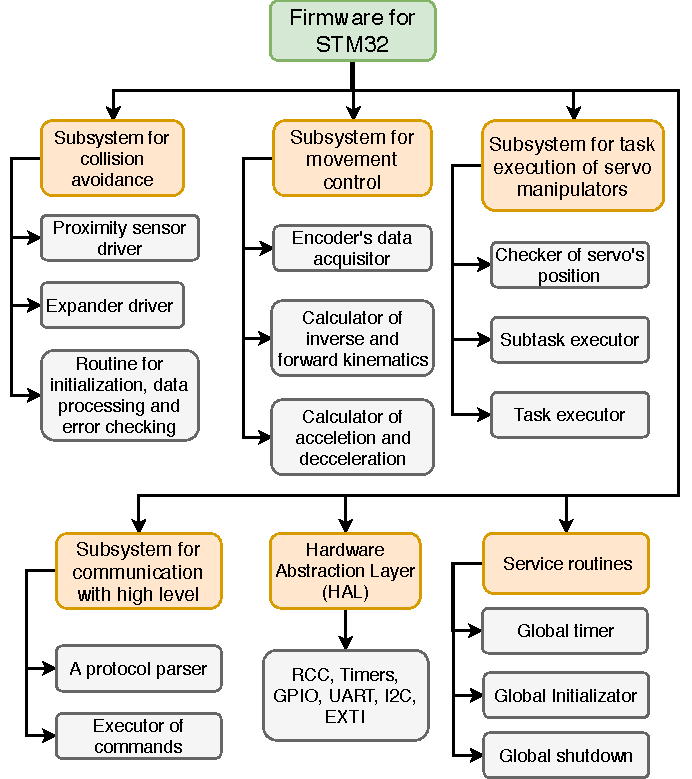
\includegraphics[scale = 1.0]
{scheme}}
\caption{The breakdown structure.}
\label{ris:scheme}
\end{figure}

\subsection{Service Routines}
There are basically three service routines that are depicted in the scheme \ref{ris:scheme}. They supports all functionality of the firmware and will be described in details in the following paragraphs. 

\paragraph{Global initialization.}

Global initialisation routine is a piece of code that performs the whole initialization of peripheral modules and sensors after a power on. To make mapping for peripheral modules more intuitive a bunch of macros are defined in \textitbf{Board.h}. Then macros are used everywhere in the firmware and especially in a function \inlinecode{void boardInitAll()} that is responsible for global initialization and is implemented in \textitbf{Board.c}

\paragraph{Global timer.}
Global timer is a main timer in the firmware that is used in all time-based functions. The quantization step of a timer is \textbf{$\textbf{1/10}$ of a millisecond}. Main three functions to work with global time are the following:
\begin{lstlisting}
uint32_t getLocalTime(void);
uint32_t getTimeDifference(uint32_t startTime);
uint8_t checkTimeout(uint32_t startTime, uint32_t timeout);
void delayInTenthOfMs(uint16_t delay);
\end{lstlisting}
The first function returns global time in tenth of a millisecond (dimension of the output is $\textbf{ms/10}$). The second function return time difference between current time and \inlinecode{startTime}. The third function returns \textitbf{1} if \textitbf{timeout} was exceeded and \textitbf{0} otherwise. The last function makes "stupid" delay for a desired time interval.
 
\paragraph{Global shutdown.}
This service routine is very important because it provides a predictable behaviour of the robot after the end of a match regardless of the high level code. The code of the function \inlinecode{void turnEverythingOff()} that is implemented in \textitbf{Robot.c} is provided below:
\begin{lstlisting}
void turnEverythingOff()
{
	// Global disable of interrupts
	
	__disable_irq();

	// Turn off dynamixels
	gpioPinSetLevel(SERVO_REBOOT_PORT, SERVO_REBOOT_PIN, 				          GPIO_LEVEL_HIGH);
	
	// Turn off maxons
	uint8_t i;
	for (i = 0x00; i < ROBOT_NUMBER_OF_MOTORS; i++)
	{
		// Change PWM
		timPwmChangeDutyCycle(motorPwmCh[i].timModule, motorPwmCh[i].channel, 0.0f);
	}
	while (1)
	{
	}
} 

\end{lstlisting}
As it can be noticed from the comments the function  turn off the interrupts globally,stops all the actuators and enters infinite cycle. The firmware call the function after successful comparison between time of robot's start and macro \inlinecode{ROBOT\_TIME\_OF\_MATCH\_TENTH\_OF\_MS} inside \textitbf{main.c}.
\subsection{Subsystem for collision avoidance}
The collision avoidance system of the robot is based on a set of proximity sensors \textitbf{VL6180X} from \textitbf{ST} company. It is a time of flight (TOF) sensor that has an approximate precision (noise) of $2\:mm$ and typical accuracy (range offset for surfaces with different reflectance) of about $13\:mm$. The sensor has digital I2C interface with a fixed I2C adress that can be changed after power on. As we are using a set of sensors with the same initial adress the subsystem also contains GPIO I2C expander \textitbf{MCP23017}. The expander allows to perform subsequent initialization of sensor's array and local reinitialization of particular sensor in case of an error. The maximum frequency of sensor's data acquisition for one sensor depends on the reflectance of the target, but it could be configured with constrained convergence time (see the datasheet for \textitbf{VL6180X}). In the firmware a custom method of sensor's initialization is used that allows to achieve $50 Hz$ data acquisition frequency and reduce the sensitivity cone for the proximity sensors. 

The source code files for  \textitbf{VL6180X} driver:
\begin{itemize}
	\item \textitbf{VL6180x.h}
	\item \textitbf{VL6180x.c}
\end{itemize}

The source code files for  \textitbf{MCP23017} driver and other subroutines:
\begin{itemize}
	\item \textitbf{Collision\_avoidance.h}
	\item \textitbf{Collision\_avoidance.c}
\end{itemize}

Periodical data acquisition of ranges is implemented in the interrupt handler of a timer called \inlinecode{COLL\_AVOID\_TIM\_MODULE}. The code of the handler is located in \textitbf{Interrupts.c}.

\subsection{Subsystem for movement control}
The subsystem for movement control is responsible for encoder's data acquisition, calculation of kinematics (inverse and forward), smooth small movements with acceleration. All necessary functions are implemented in source code files:
\begin{itemize}
	\item \textitbf{Robot.h}
	\item \textitbf{Robot.c}
\end{itemize}

The functions are separated into several groups. A short description of each function can be found in table \ref{tab:functions_for_movement}.

\begin{longtable}[H]{|m{6 cm}|m{7 cm}|}
\caption{ Functions of the subsystem for movement control}\label{tab:functions_for_movement}\\
\hline
\multicolumn{1}{|c|}{Function} & \multicolumn{1}{|c|}{Short description} \\
\hline

\multicolumn{2}{|c|}{\textitbf{Odometry data acquisition}} \\
\hline
\inlinecode{readEnc (void)} & Reads data from encoders, calculate coordinates and speeds of each wheel, calculates instanteneous coordinates and speeds in robot's coordinate system. \\
\hline
\inlinecode{calcGlobSpeedAndCoord (void)}& Calculates robot's speed components and coordinates in global coordinate system by using speeds in robot's coordinate system.\\
\hline

\multicolumn{2}{|c|}{\textitbf{Motor control}} \\
\hline
\inlinecode{setMotorSpeed (uint8_t motorNumber, float speed)} & Sets speed of particular wheel. It is comfortable to use for diagnostics. \\
\hline
\inlinecode{setMotorSpeeds (void)} &Sets received target speeds for all motors. \\
\hline

\multicolumn{2}{|c|}{\textitbf{Calculation of kinematics}}\\
\hline
\inlinecode{calcForwardKin (void)}  & Calculates forward kinematics (from speeds in robot's coordinate system to motors' speed).\\
\hline
\inlinecode{checkSaturation (float* targetSpeed)} & Check saturation of motors and change speeds if it is needed (speeds in robot's coordinate system).\\
\hline
\inlinecode{calcInverseKin (void)} & Calculates inverse kinematics (from wheels' speeds to speeds in robot's coordinate system).\\
\hline

\multicolumn{2}{|c|}{\textitbf{Movement with acceleration}}\\
\hline
\inlinecode{startMovementRobotCs1 (float* distance, float* speedAbs, float accelerationAbs[3])} & Starts short distance movement with acceleration in robot's coordinate system. Input accelerations are corrected inside the function in order to be syncronized.\\
\hline
\inlinecode{calculateTrajectParameters (uint8_t coordinateNumber, float* accelerationAbs)} & Inner function for calculation of points of accelleration and decceleration.\\
\hline
\inlinecode{syncAccelerations (float* distance, float* speedAbs, float* accelerationAbs)} & Inner function for syncronizing accelerations.\\
\hline
\inlinecode{speedRecalculation (void)} & Speed recalculation based on current speed and coordinate in robot's coordinate system.\\
\hline
\inlinecode{checkIfPositionIsReached (void)} & Function checks if we reached desired position or not and changes mode of movement when the robot reaches transition points.\\
\hline
\inlinecode{checkIfPositionIsReachedCoord (uint8_t i, float* robotCoordBuf)} & Subfunction for previous function.\\
\hline
\end{longtable}

An implementation of the particular function should be clear from the source code. However, a short description of movement with acceleration should be provided. Firstly, this feature is implemented to provide short and precise displacements of the robot. Therefore robot's coordinate system is used as a reference. When a high level sends a command for a short displacements, the firmware calls the function \inlinecode{void startMovementRobotCs1(float* distance, float* speedAbs, float accelerationAbs[3])}. Arguments of the function are distances (\textitbf{x, y, angle}), absolute speeds that robot should reach after acceleration and absolute values of accelerations. Inside the function \inlinecode{void startMovementRobotCs1(...)} the following sequence of steps are implemented:
\begin{enumerate}
\item \textitbf{Normalization of absolute speeds}

(Absolute speeds are converted into motors' speeds and scaled if the values exceed maximum speed);
\item \textitbf{Normalization of accelerations}

(Absolute accelerations are scaled to make the time of acceleration and deceleration for all coordinates equal. It is necessary to keep the direction of movement constant during acceleration/deceleration);
\item \textitbf{Filling of the struct for odometry movement with necessary parameters}

(This step resets the coordinates in robot's system to zero, assign right signs for speed and acceleration, based on input distances. Moreover it optimizes the rotation based on input target angle, calculates speeds' increments, coordinates of points, where acceleration should stop and where deceleration should start).
\end{enumerate}

After the initialization in the interrupt handler of motor control timer firmware calls the function \inlinecode{checkIfPositionIsReached (void)} to check if the robot has already reached destinations point \textbf{OR} if it is time to start stable movement / deceleration \textbf{OR} if the timer is expired. Then the firmware calls \inlinecode{void speedRecalculation(void)} to recalculate speeds depending on the current step.


Apart from the functions mentioned in the table \ref{tab:functions_for_movement} there are some supplementary funtions for matrix calculations (see \textitbf{Matrix.c}, \textitbf{Matrix.h}), angle normalization (see \inlinecode{static void normalizeAngle(float* angle)} of \textitbf{Robot.h})) and other trivial procedures.

\subsection{Subsystem for task execution of servo manipulators}

\subsection{Subsystem for communication with high level}

\subsection{Hardware abstraction layer (HAL)}

%\section*{\hfil Instructions \hfil}

%    \begin{lstlisting}
%	typedef union {
%		uint64_t raw;
%		struct {
%				uint8_t prescaler;
%				uint32_t clock;
%				uint16_t comp;
%				};
%	} timer_desc;
%	\end{lstlisting}

\end{document} % конец документа

